\chapter{Description}
 
 A detailed list of procedures to build and prepare environment to develop \emph{EduXes} application, will be described.
 Also a description of how development was carried out, step by step are show.
 

\section{Preparation of development}
Firstly Java Development Kit (JDK) version 1.6 is needed, to build application itself and the Eclipse IDE, is downloaded from \emph{Oracle}: 
\cite{JavaSE}
\begin{quote}
\url{http://www.oracle.com/technetwork/java/javase/downloads/index.html}
\end{quote}

As root user downloaded file is unpacked into {\bf /usr/lib/jvm } and configured to be the Java default:
%%  \begin{bclogo}[couleur=green!30,arrondi=0.1, logo=\bcpanchant,  ombre=true ] 
\begin{bclogo}[couleur=red!30,arrondi=0.1, logo=\bcpanchant,  ombre=true ] 
{Update Java}   
\begin{verbatim}
 # update-java-alternatives -s JDK_1.6_NAME
\end{verbatim}
\end{bclogo}

	\emph{Eclipse Juno (4.6)} is downloaded from its site \cite{Eclipse}: $Download \rightarrow Linux \, 64\, bits$
\begin{quote}
\url{http://www.eclipse.org}
\end{quote}
Android Development Toolkit (ADT)\cite{AndroidDevelopmentKit} is downloaded following instructions on this page:
\begin{quote}
\url{http://developer.android.com/sdk/installing/installing-adt.html}
\end{quote}

	In Eclipse a new line is included into repository software ($Help \rightarrow  Install\, New\, Software \rightarrow Add$):
\begin{quote}
\url{http://dl-ssl.google.com/android/eclipse/}
\end{quote}
	Next step is to select all the related software listed.
	
	For Aptana Plugin the line to be added into Eclipse is: 
\begin{quote}
\url{http://download.aptana.com/studio3/plugin/install}    
\end{quote}

	Furthermore JQuery, JQueryMobile and Phonegap are needed, and were downloaded from their web sites:
	\begin{itemize}
	    \item {JQuery 1.8.1} (no newer versions), from \url{http://jquery.com/} :
	    \subitem JQuery will be  copied into {\bf assets/www/js} folder.
	    \item {JQueryMobile 1.1.1} from \url{ http://jquerymobile.com/}: 
        \subitem JQueryMobile is a zip file which will be uncompressed and copied into  {\bf assets/www/js} folder.
        \item{PhoneGap - Cordova 1.8.1} is downloaded from \url{https://github.com/phonegap/phonegap/zipball/1.8.1}
        and installed following reference \cite{PhoneGapGS} 

	\end{itemize}

	To create a PhoneGap application there are very important instructions (Getting Started with Android)  should be followed step by step:
\cite{AndroidGettingStarted}
\section{Application Skeleton}
  Next step is to choose application name and folders policy. Name \emph{EduXes} stands for "Educaci\'n" and "Xesti\'on", is a educational management software.
About folders policy, a folder is created ({\bf assets/www/js}) which contains javascript ({\bf *.js}) files except \emph{JQuery} and \emph{JQueryMobile} which is included into another
 folder ({ \bf assets/www/js/jquery} ), do not forget style sheets files ({\bf *.css } )
 
To finish building application skeleton a simple application is created which contains only a blank page.
 
Getting started with Android \cite{AndroidGettingStarted} is followed step by step.

\section{Upload into Git repository}

 Following stage is to upload that simple application into a git repository. 
An account is created in Github\cite{GitHub}, which is the largest code host in the world,  and a new application is initialized.  This are the source code project page \url{https://github.com/joseantoniosa/EduXes}.

Then source code are upload to Github: 

  \begin{bclogo}[couleur=green!30,arrondi=0.1, logo=\bcpanchant,  ombre=true ] 
{Git init shell}   
\begin{verbatim}
$ git init
$ git add -A *
$ git remote add  EduXes git@github.com:joseantoniosa/EduXes.git 
$ git push origin master
\end{verbatim}
\end{bclogo}

Each time an update in code is done,  code is uploaded :

  \begin{bclogo}[couleur=green!30,arrondi=0.1, logo=\bcpanchant,  ombre=true ] 
{Git update}   
\begin{verbatim}
$ git add -A *
$ git commit -m 'CHANGES_DESCRIPTION'
$ git push origin master
\end{verbatim}
\end{bclogo}

\newpage
\section{Development}
 Before begining with development itself is compulsory to explain some concepts already shown above in Methodology (\ref{Methodology}), but with more detail:
JQueryMobile \cite{JQueryMobile} and by extension,  PhoneGap \cite{PhoneGap}  applications, are structured in pages:
 \begin{quote}
  <div data-role="page">
 \end{quote}

   which are very similar to desktop applications windows. Therefore, from Javascript code, to change to a new page 
\begin{quote}
 \$.mobile.changePage("\#daily\_work");
\end{quote}
       opens \textit{"daily\_work"} page.  
     
% Application Work-flow 
% Next illustration try to be self-explicative.  Beginning at onDeviceReady()  from interface.fs file.  Inside each page several actions are performed: e.g., open and populate database, load list of groups (loadSchedule()),  and user choose next step according options shown. 
% 
% 
% %%%%%%%%%%%%%%%%%%%%%%%%%%%%%%%%%
% 
% 
% Development:
As shown before (\ref{Methodology}) \emph{EduXes} contains several files:
\begin{itemize}
\item Four files contain application code:
\subitem  {\bf interface.js} : It contains information and decisions related to interface and application workflow, completely independent from database. It is located in {\bf assets/www/js} folder.
\subitem { \bf database.js} : It contains database related code: SELECT, INSERT, etc. It is located in {\bf assets/www/js} folder.
\subitem {\bf index.html}, {\bf remove.html} only contain HTML framework, page properties, and static content.  They are located in {\bf assets/www/} folder.
\item There are three important files which contain documentation:
\subitem {\bf TODO.txt}. List of goals to be achieved and milestone reached. It is located in root application folder.
\subitem {\bf DATABASE.sql}.  Data-base structure in SQL format. This file are shown below. It is located in root application folder.
\subitem {\bf REAME.txt}. Only contains general information about this application.It is located in root application folder.
\end{itemize}

Also, \emph{Eclipse} generates several files, the most important is the application file, which is an {\bf apk } package: {\bf bin/EduXes.apk}.

Next step is to build database, this will be described below \ref{DataBase}. 
Following database, sample data is needed to begin application development. 

\newpage

\subsection{Groups}

The first window to be developed is \emph{List of Groups}: as shown above \ref{Methodology}, firstly a \emph{page} is created inside {\bf index.html}. This page, as every page,  has three important elements:
\begin{itemize}
    \item  \emph{header}. It could contain a backward button, which return application flow to previous visited page. This is disabled,
because it could cause problems when previous page is an edit page, and another solution is preferred.    
    \item \emph{content}. Data itself, it has an important \emph{id} to be filled with content by javascript code.
    \item \emph{footer}. Usually page name.
\end{itemize}

\begin{figure}
    \begin{center}
%%            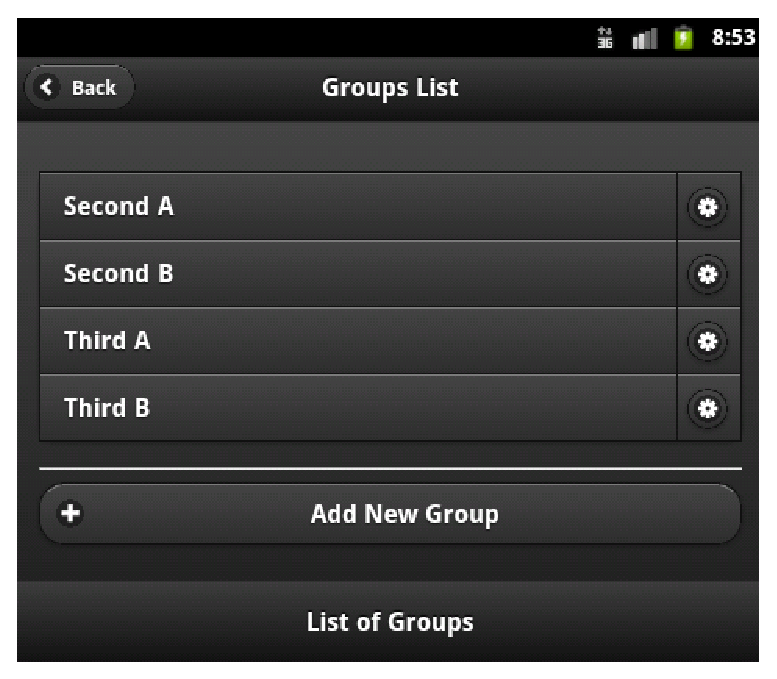
\includegraphics[width=\textwidth]{eduxes_groups_list.eps}
        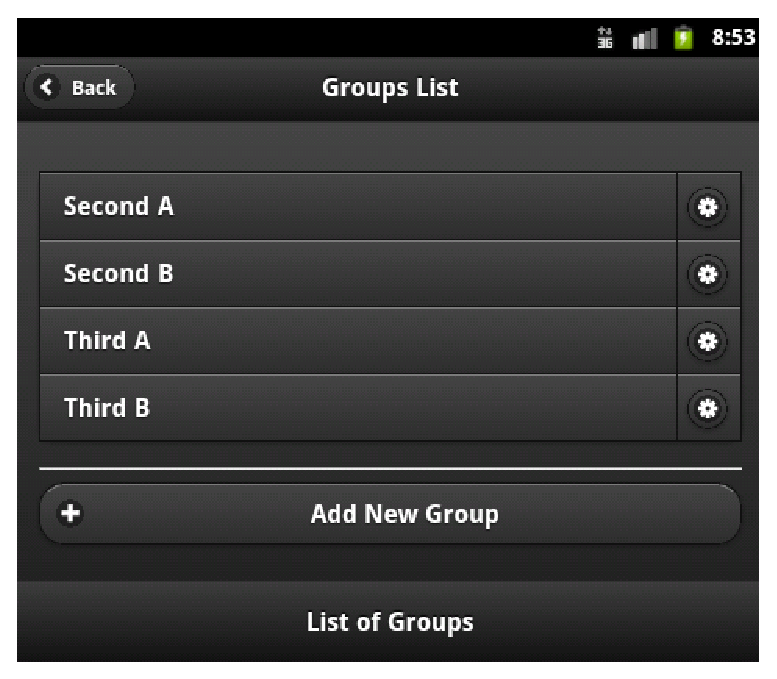
\includegraphics{eduxes_groups_list.eps}
        \caption{List of Groups}
        \label{fig:EduXesGroups}
    \end{center}
\end{figure}



\begin{bclogo}[couleur=blue!30,arrondi=0.1,ombre=true ] 
%% \begin{bclogo}[couleur=blue!30,arrondi=0.1, logo=\bcpanchant, barre=zigzag,  ombre=true ] 
{List Groups page. index.html}
\begin{verbatim}
<div data-role="page" id="list_groups" data-add-back-btn="true">
    <div data-role="header"  data-add-back-btn="false"  >
        <a href="#list_settings"  data-icon="arrow-l"
             data-theme="a" data-role="button">Back</a>
        <h1>Groups List</h1>
    </div>                
    
    <div data-role="content">
    <ul id="groups_ul" data-role="listview" data-inset="true"  
        data-split-icon="gear" data-split-theme="a" >
    </ul>
     <hr />
     <a  style="text-align: center" onClick="onAddNewGroup();" 
        data-role="button" data-icon="add">Add New Group</a>
    </div>
    <div data-role="footer"  data-rel="back" data-theme="a">
     <p style="text-align: center">List of Groups</p>
    </div>
</div>
\end{verbatim}
\end{bclogo}
To fill this list of elements \emph{<ul id=groups\_ul (...)>} a function \emph{onListAllGroups()} is called. 

Firstly a \texttt{loading ...} logo appears, then a function from {\bf database.js} is called (\emph{loadAllGroups() }).
\begin{bclogo}[couleur=blue!30,arrondi=0.1,ombre=true ] 
{List Group page. interface.js}
\begin{verbatim}
function onListAllGroups(){
    $.mobile.showPageLoadingMsg();
    table_global='GROUPS';
    loadAllGroups(global_db); // #groups_ul
    $.mobile.changePage("#list_groups", { transition: "slideup"} );
}
\end{verbatim}
\end{bclogo}

Function (\emph{loadAllGroups() }) calls (\emph{queryAllGroupsDB()}) from \texttt{database.js}. 
This function fills \textit{\$('\#groups\_ul')}  combo box with group data: \textit{name}. Moreover user
can access  a list of students of that group (\textit{listStudentsByGroup()}) or change
group information (\textit{EditGroup()}).


\begin{bclogo}[couleur=blue!30,arrondi=0.1,ombre=true ] 
{List Group page. database.js}
\begin{verbatim}
function queryAllGroupsDB(tx) {
    log("Query All Groups \n");
    var ul_list =$('#groups_ul');
    tx.executeSql('SELECT * FROM GROUPS', [],
        dbSuccessFunc = function(tx, rs) {
        ul_list.empty();
        var html ="";
        for (var i = 0; i < rs.rows.length; i++) {
          id = rs.rows.item(i).id ;
          html = "<li>";
          html += "<a onClick='global_id=" + id + 
              "; global_id_group="+id
              +"; table_global=\"groups\"; ";
          html += " listStudentsByGroup(" + id + " );'  ";
          html += " href='#' >";
          html += rs.rows.item(i).data;
          html += "</a>";
          html += " <a data-role='button' data-position-to='window'";
          html += " data-iconpos='notext' ";
          html += " style='float:right;' href='#' ";
          html += " data-rel='dialog' data-theme='a' ";
          html += " data-transition='slideup' ";
          html += " onClick=\"EditGroup(" + id + "); ";
          html += " global_id_group="+id
              +"; global_id=" + id + "; \">Edit</a>";
          html +="</li>";
          ul_list.append(html);
        }
        ul_list.listview('refresh'); },
        dbErrorFunc = function(ttx, e) {
            if (ttx.message)
                e = ttx;
            log(" There has been an error Select * from groups : " 
            + e.message);
        return false;
    });
}
\end{verbatim}
\end{bclogo}


Second window to be developed is edit group information. The contents of \textit{Edit Group} page from \textbf{index.html} is
filled by loadGroup() function \textbf{database.js} as shown below \ref{edit_group_database}.

\begin{bclogo}[couleur=blue!30,arrondi=0.1,ombre=true ] 
{Edit Group page. index.html }
\begin{verbatim}
<div data-role="page" id="edit_groups" data-add-back-btn="true">
    <div data-role="header"  data-add-back-btn="true" >
        <h1>Group Edition</h1>
    </div>
    <div data-role="content">
        <label for="nombre_grupo">Name</label>
        <input id="in_nombre_grupo" enabled="true" />
        <label for="nivel_grupo">Level</label>
        <input id="in_nivel_grupo" enabled="true" />
        <a onClick="onUpdateGroup();" data-role="button" 
            data-icon="check">Save</a>
	</div>
</div>
\end{verbatim}
\end{bclogo}

\begin{bclogo}[couleur=blue!30,arrondi=0.1,ombre=true ] 
{Edit Group page. interface.js}
\begin{verbatim}
function EditGroup(id_group){
    $.mobile.showPageLoadingMsg();
    global_id = id_group;      //local variable goes global
    table_global = 'GROUPS';
    loadGroup(global_db,id_group);
    $.mobile.changePage("#edit_groups", { transition: "slideup"});
}
\end{verbatim}
\end{bclogo}

Inside \textit{loadGroup} function a sql query is built \texttt{(SELECT ... FROM ...)}, then
it is executed and returned values are loaded in result set variable (\textit{rs}). 
With this data html form  is populated (\textit{\$('\#in\_nombre\_grupo')}). 
Whether an error is triggered then \textit{dbErrorFunc} is called an a message appears on user interface.

These procedures will be very similar to all \textit{"load"} functions (students, activities).

\begin{bclogo}[couleur=blue!30,arrondi=0.1,ombre=true ] 
{Load Group page. database.js  \label{edit_group_database}}
\begin{verbatim}
function loadGroup(db, id_group){
    db.transaction(function (tx) {
        log("Query Group \n");
        var sql = 'SELECT id, data, other_data ':
        sql += ' FROM GROUPS WHERE id ='+id_group;
        tx.executeSql(sql, [],
            dbSuccessFunc = function(ttx,rs){
                $('#in_nombre_grupo').val(rs.rows.item(0).data);
                $('#in_nivel_grupo').val(rs.rows.item(0).other_data);
            },
            dbErrorFunc = function(tx, e) {
                if (tx.message) e = tx;
                    log(" There has been an error queryGroupDB: " 
                        + e.message);
                    alert(" There has been an error queryGroupDB: " 
                        + e.message);
                    return false;
            });
    });
}
\end{verbatim}
\end{bclogo}


\newpage
\subsection{Students}    

Students pages are very similar to groups but, obvously, contain different fields (a complete list of fields is shown in database
definition \ref{DataBase}). Only list of students by group page and \textit{LoadStudentsByGroup} code are shown. 
They are very similar to their \textit{groups} counterpart. The main concern is about escape characters and colons,
code is straightforward to read. Several lines were removed towards readability \textit{(...)}. 

\begin{figure}
    \begin{center}
        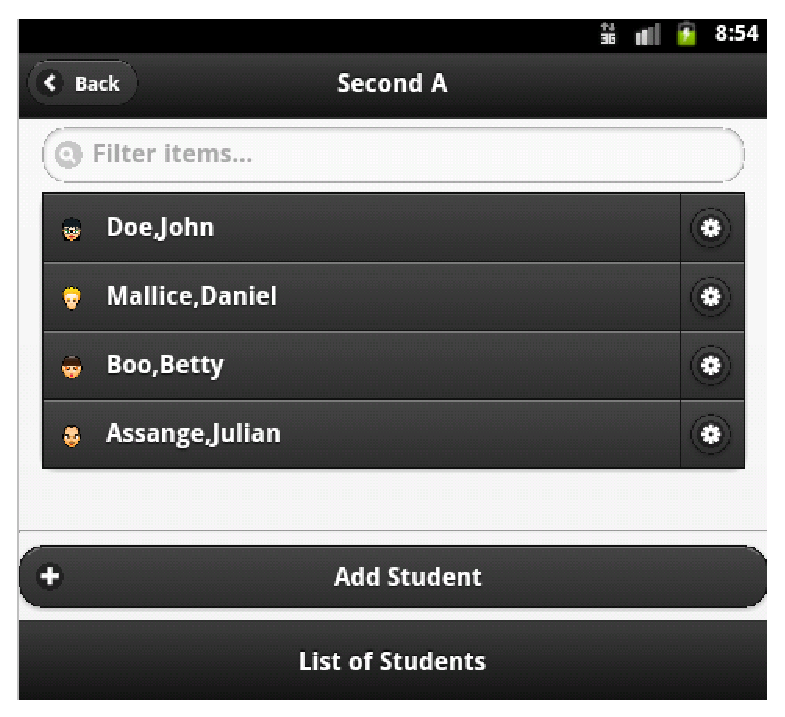
\includegraphics{eduxes_list_students.eps}
        \caption{Students}
        \label{fig:EduXesStudents}
    \end{center}
\end{figure}


\begin{bclogo}[couleur=blue!30,arrondi=0.1,ombre=true ] 
{List Students page. index.html \label{list_students_page}}
\begin{verbatim}
<div data-role="page" id="list_students_by_group" 
    data-add-back-btn="true">
    <div data-role="header"  data-back-btn-text="previous" 
        data-add-back-btn="true" >
        <h1 id="id_list_students_by_group"> Students List</h1>
    </div>
    <div data-role="content">
        <ul id="list_students_by_group_ul" data-role="listview" 
        data-theme="a" data-split-theme="a" data-split-icon="gear" 
        data-filter="true" data-inset="true"  >
        </ul>
    </div>
    <hr />
    <a onClick="onAddNewStudent();" data-role="button" 
    data-icon="add"  data-theme="a" >Add Student</a>
    <div data-role="footer" class="footer-docs" data-rel="back" 
    data-theme="a">
        <p style="text-align: center">
            List of Students
        </p>
    </div>
</div>
\end{verbatim}
\end{bclogo}


\newpage


\begin{bclogo}[couleur=blue!30,arrondi=0.1,ombre=true ] 
{Load Student snippet. database.js  \label{load_student_database}}
\begin{verbatim}
function loadStudentsByGroup(db,id_group) {
 db.transaction(
  function (tx) {
   var sql = 'SELECT STUDENTS.id as id, ';
   sql += ' STUDENTS.id_group as id_group,';
   sql += ' STUDENTS.name as name, ';
   (...)
   sql += ' FROM STUDENTS, GROUPS WHERE ';
   sql += ' STUDENTS.id_group = g_id AND id_group=';
   sql += ' + id_group;
   tx.executeSql(sql, [],
    dbSuccessFunc = function(tx, results) {
     var len = results.rows.length;
     var ul_list = $('#list_students_by_group_ul');
     $('#id_list_students_by_group').text(
        results.rows.item(0).data );
     var html;
     ul_list.empty();
     var id = 0;
     for (var i = 0; i < len; i++) {
        id = results.rows.item(i).id;
        html="<li >";
        html+="<a onClick='global_id="+id;
        html+=";table_global=\"students\";'"; 
        html+=" href='#' data-rel='dialog' ";
        html+=" data-transition='slideup'>";
(...)
        html+=results.rows.item(i).surname + "," ;
        html+=results.rows.item(i).name+"</a>";
        html+="<a data-role='button' "; 
        html+=" data-position-to='window' ";
        html+=" data-iconpos='notext' "; 
        html+=" style='float:right;' href='#' ";
        html+=" data-rel='dialog' ";
        html+=" data-transition='slideup'  ";
        html+=" onClick=\"EditStudent(" ;
        html+=id + ");\">Edit</a> </li>";
        ul_list.append(html);
    }
    ul_list.listview('refresh'); },
    dbErrorFunc = function(tx, e) {
     if (tx.message) e = tx;
     log(sql);
     log(" Error loadStudentsByGroup: "+e.message);
     alert("Error loadStudentsByGroup: " + e.message);
     return false;
    });
    }
   );
}
\end{verbatim}
\end{bclogo}

\newpage

\subsection{Main Page}

Main page was not the very first page to be built, because it is related with attendance, sessions, groups and students, and also reports.
Its design it has to follow several basic principles: simple but with no more than four clicks (even less)away to 
 access to every application window-page. The most important item is current data, and the \textit{">" } symbol on the right to access \textit{Attendance} page.
 
 There are a table with three columns (\textit{class="ui-grid-b"}), which contains a label, the current date, and an info button.
 And a list of navigation buttons to list data (\texttt{report}) or manage students, groups and activities (\texttt{settings})
 
Of course there are a lot of elements that could be changed to improve user experience in this page.

\begin{figure}
    \begin{center}
        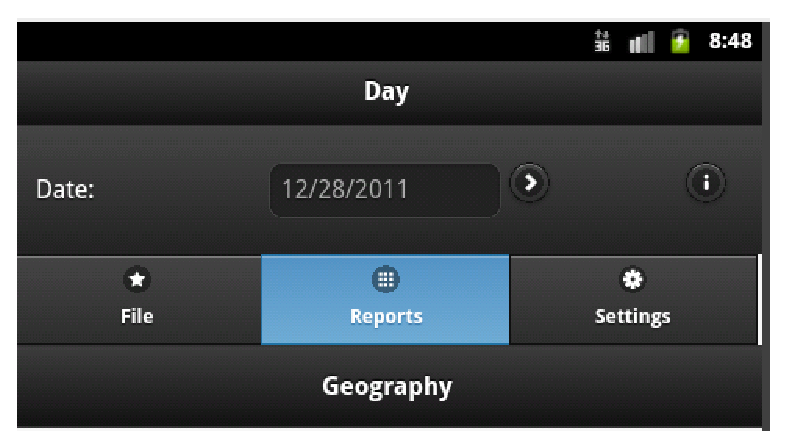
\includegraphics{eduxes_main_page1.eps}
        \caption{Main Page}
        \label{fig:EduXesMainPage}
    \end{center}
\end{figure}


\begin{bclogo}[couleur=blue!30,arrondi=0.1,ombre=true ] 
{Main Page. index.html \label{main_page}}
\begin{verbatim}
<!-- Main Window    //-->
<div data-role="page" id="daily_work">
    <div data-role="header" data-add-back-btn="true" data-theme="a">
        <h1>Day</h1>
    </div>
    <div data-role="content" data-theme="a">
        <div class="ui-grid-b">
        <div class="ui-block-a">
            <div data-role="fieldcontain">
                <label for="date"  >Date:</label>
            </div>
        </div>
        <div class="ui-block-b">
            <input id="daily_date_scroller" 
            name="daily_date_scroller" />
        </div>
        <div class="ui-block-c">
            <a href="#" data-role='button' 
            data-icon='info' data-iconpos='notext' 
            style='float:right;' onClick="help('date');">Help</a>
            <a href="#" data-role="button" 
            data-icon="arrow-r" data-iconpos="notext"  
            onClick="open_daily_page() " >Go</a>
        </div>
    </div>
    </div>
    <div data-role="navbar">
        <ul>
            <li>
                <a href="#" onClick="onGeneralFile()  "  
                data-role="button" data-icon="star"  
                data-theme="a" > File</a>
            </li>
            <li>
                <a href="#" onClick="onGeneralListReports();"  
                data-role="button" data-icon="grid"  
                data-theme="a" >Reports</a>
            </li>
            <li>
                <a href="#" onClick="onGeneralListSettings();" 
                data-role="button" data-icon="gear"   
                data-theme="a" >Settings</a>
            </li>
        </ul>
    </div><!-- /navbar -->
    <div data-role="footer" class="footer-docs" data-theme="a">
        <p   style="text-align:center;"  id="teachers_name"></p>
    </div>
</div>
\end{verbatim}
\end{bclogo}

\newpage
\subsection{Attendance}

\begin{figure}
    \begin{center}
        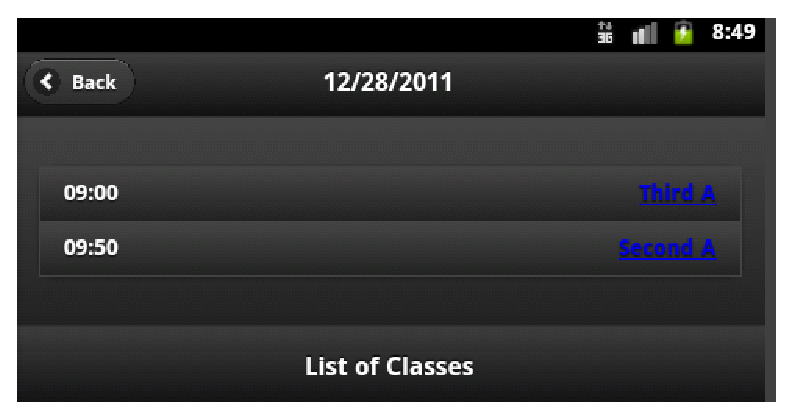
\includegraphics{eduxes_schedule1.eps}
        \caption{Schedule}
        \label{fig:EduXesSchedule}
    \end{center}
\end{figure}




\texttt{Attendance} per group is one of most important pages, and it list attendance, behaviour of 
students of a group. There is a previous page: list of groups for current day (\textit{Schedule page})
(Figure: \ref{fig:EduXesSchedule}) \ref{schedule_page}.

\begin{bclogo}[couleur=blue!30,arrondi=0.1,ombre=true ] 
{Schedule Page. index.html \label{schedule_page}}
\begin{verbatim}
<div data-role="page" id="daily_schedule"  
 data-add-back-btn="false"  data-theme="a" >
    <div data-role="header"  
        data-back-btn-text="previous" 
        data-add-back-btn="false" data-theme="a">
        <a href="#daily_work"  
        data-icon="arrow-l" data-theme="a" 
        data-role="button">Back</a>
        <h1 id="current_day"> Current Day</h1>
    </div>
    <div data-role="content" data-theme="a">
        <ul id="groups_day_ul" data-role="listview" 
        data-inset="true" data-split-icon="gear"  
        data-split-theme="a" >
        </ul>
    </div>
    <div data-role="footer" class="footer-docs" 
        data-add-back-btn="true" data-theme="a">
        <p  style="text-align:center;" > List of Classes</p>
    </div>
</div>
\end{verbatim}
\end{bclogo}

\begin{figure}
    \begin{center}
        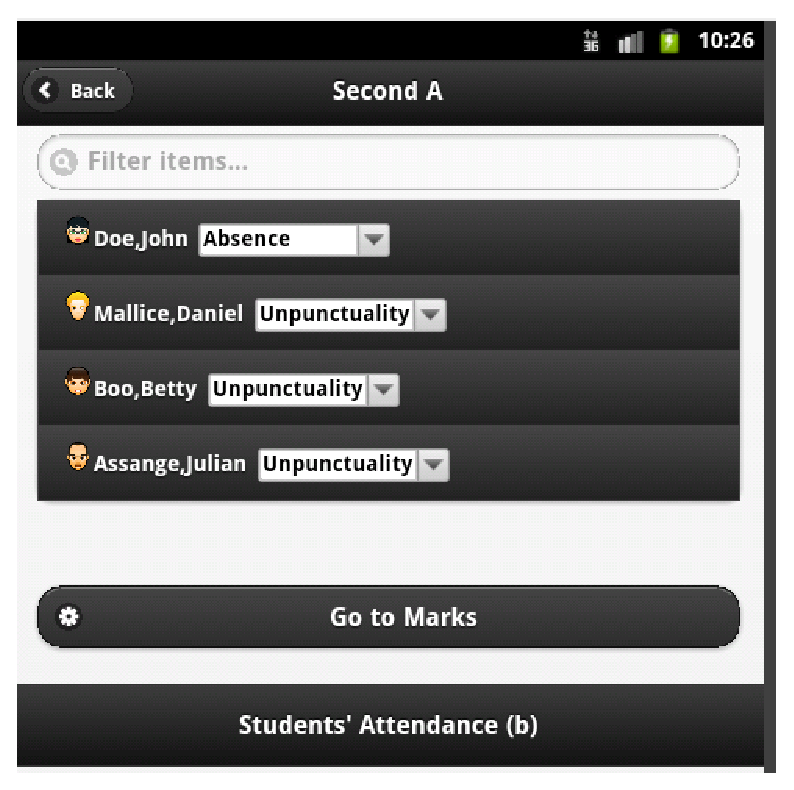
\includegraphics{eduxes_students_attendance2.eps}
        \caption{Attendance}
        \label{fig:EduXesAttendance}
    \end{center}
\end{figure}

The \textit{queryStudentsAttendanceSuccess} \ref{attendance_student} function fills \textit{Attendance} page \ref{attendance_page} with photos, names and surnames
of student of the adequate group. User can choose among different student "states", these "states" are filled in
\textit{fillSelectStudent} function. When user changes combo values function \textit{studentState} is called which
update or insert student state into \textit{attendance} table in database.

\begin{bclogo}[couleur=blue!30,arrondi=0.1,ombre=true ] 
{Attendance Page. index.html \label{attendance_page}}
\begin{verbatim}
<div data-role="page" id="list_students_attendance" 
    data-add-back-btn="false">
    <div data-role="header"  data-back-btn-text="previous" 
        data-add-back-btn="false"  data-theme="a" >
        <a href="#" onClick="open_daily_page();" data-icon="arrow-l" 
            data-theme="a" data-role="button">Back</a>
        <h1 id="current_group_attendance">Student List for Group</h1>
    </div>
    <div data-role="content"> <!---Data goes here //-->
        <ul data-role="listview" id="students_attendance_ul" 
        data-autodividers=!"true" data-split-icon="gear" 
        data-split-theme="a" data-filter="true" data-inset="true" 
        data-theme="a" ></ul>
    </div>
    <div data-role="content">   
    <a href="#" onClick="onOpenStudentsAssessment();" 
    data-icon="gear" data-theme="a" 
    data-role="button">Go to Marks</a>
    </div>
    <div data-role="footer" class="footer-docs" 
    data-rel="back" data-theme="a">
        <p style="text-align:center;"  >Students' Attendance (b)</p>
    </div>
</div>
\end{verbatim}
\end{bclogo}


\begin{bclogo}[couleur=blue!30,arrondi=0.1,ombre=true ] 
{Fill Attendance database.js \label{attendance_student}}
\begin{verbatim}
function queryStudentsAttendanceSuccess(tx, results) {
  (...)
  for (var i=0;i<results.rows.lengthi++) {
    id = results.rows.item(i).id_student;
    photo = results.rows.item(i).photo;
    name = results.rows.item(i).name;
    surname = results.rows.item(i).surname;
    id_group = results.rows.item(i).g_id;
    id_session = global_session; //
    html = "<li data-role='fieldcontain'> ";
    html+= "<label for='select_student_"+id+"' class='select'>";
(...)
    html+= surname + "," + name + "</label> " ;
    html+="<select name='select_student_"+id
        +"' id='select_student_"+id+"' ";
    html+= " onChange='studentState("+id + "," 
        +id_group + ","+id_session+ ");'>";
    html+="</select>";
    html+= "</li>";
    $('#students_attendance_ul').append(html);
    fillSelectStudent(global_db,"select_student_"+id,id_session,id);
  } 
  $('#students_attendance_ul').listview('refresh');
}
\end{verbatim}
\end{bclogo}

\begin{figure}
    \begin{center}
        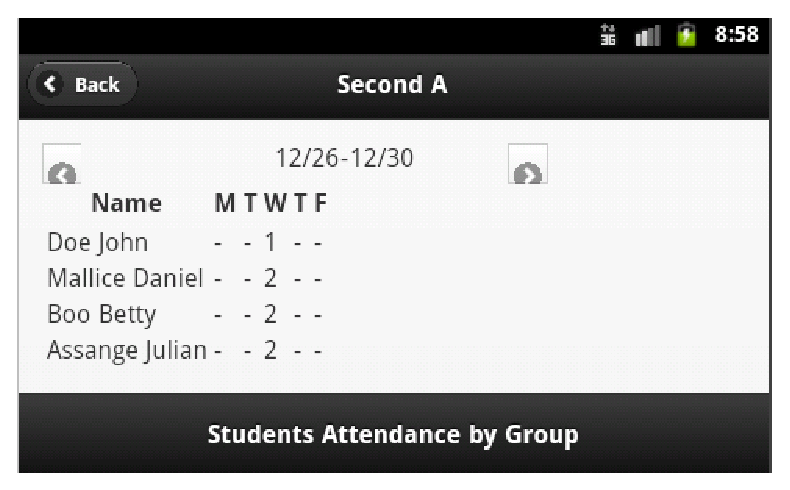
\includegraphics{eduxes_reports_attendance1.eps}
        \caption{Attendance Report}
        \label{fig:EduXesAttendanceReports}
    \end{center}
\end{figure}

\newpage
\subsection{Activities}   

Activities list is very similar to groups and students.
\begin{bclogo}[couleur=blue!30,arrondi=0.1,ombre=true ] 
{List Activities: index.html \label{activities_list}}
\begin{verbatim}
<div data-role="page" id="list_all_activities" name="activities"
   data-add-back-btn="false"  data-direction="reverse"  
   data-theme="a" >
    <div data-role="header"  data-add-back-btn="false" >
    <a href="#list_settings"  data-icon="arrow-l" data-theme="a" 
    data-role="button">Back</a>
            <h1>List of Activities</h1>
    </div>
    <div data-role="content">
                <h2 data-role="listview" 
                    id="header_activities"  ></h2>
                <ul data-role="listview" 
                    id="activities_ul"  ></ul>
    </div>
    <div data-role="footer" class="footer-docs" data-rel="back" 
        data-theme="a">
            <a onClick="onAddNewActivity();" data-role="button" 
                data-icon="add">Add New Activity</a>
            <p style="text-align: center"> List of Activities</p>
    </div>
</div>
\end{verbatim}
\end{bclogo}
\newpage

Javascript code for list of activities \ref{load_all_activities} is similar to their students and groups counterparts.

\begin{bclogo}[couleur=blue!30,arrondi=0.1,ombre=true ] 
{Load all activities: database.js \label{load_all_activities}}
\begin{verbatim}
function queryLoadAllActivitiesDB(tx) {
 tx.executeSql('SELECT * FROM ACTIVITIES',[],
  dbSuccessFunc = function(tx, results) {
    var len = results.rows.length;
    if(len>0) {
        var ul_list = $('#activities_ul');
        var html;
        ul_list.empty();
        var id = 0;
        for (var i = 0; i < len; i++) {
            id = results.rows.item(i).id;
            html = "<li >";
            html += "<a onClick='global_id=" + id + "; 
            table_global=\"activities\";
              onUpdateActivity("+id+") ' ";
            html +=  " href='#' data-rel='dialog'
             data-transition='slideup'>";
            html += results.rows.item(i).name ;
            html += "</a>";
            html += "<a data-role='button' 
                data-position-to='window' ";
            html += " data-iconpos='notext' 
                style='float:right;' href='#' ";
            html += " data-rel='dialog' 
                data-transition='slideup'  ";
            html += " onClick=\"onUpdateActivity(" +
                 id + ");\">Edit</a>";
            html += "</li>";
            ul_list.append(html);
        }
        ul_list.listview('refresh');
        global_max_activities = results.rows.length;
        }
        },
        (...)
  );
}
\end{verbatim}
\end{bclogo}
Function \textit{loadActivity} is more complex that student or groups because
when an  activity is updated, information about groups (name) is compulsory to determine 
whether a group will carry out that activity.


\begin{bclogo}[couleur=blue!30,arrondi=0.1,ombre=true ] 
{Load Activity: database.js \label{load_activity}}
\begin{verbatim}
function loadActivity(db, id_activity ) {
var sql = " SELECT  id, name , date_init , date_end , 
 weight , final FROM ACTIVITIES WHERE id="+id_activity;
 db.transaction(function(tx) {
  tx.executeSql(sql,[],
   dbSuccessFunc = function(tx, results) {
    if(results.rows.length>0 ){
     $('#in_name_activity').val(results.rows.item(0).name);
(...)
     var sql= "SELECT id, data, other_data FROM groups;";
     tx.executeSql(sql,[],
      dbSuccessFunc = function(ttx, rs) {
       if(rs.rows.length>0) {
(...)
        for (var i = 0; i < rs.rows.length; i++) {
                   id = rs.rows.item(i).id;
                    html = "<li >";
(...)
                    html += rs.rows.item(i).data +"</label>";
                    html += " </li></br>";
                    ul_list.append(html);
        }
        var sql = "SELECT  activities_group.id_group,
             activities_group.id_activity, ";
(...)
        tx.executeSql(sql,[],
            dbSuccessFunc = function(txx, rrs) {
                for (var i = 0; i < rrs.rows.length; i++) { 
                    var id_group = rrs.rows.item(i).id_group;
                    var in_act = $("#in_group_activity_" + id_group );
                    if(rrs.rows.item(i).enabled !=0) {
                         in_act.attr("checked",true); 
  (...)
}
\end{verbatim}
\end{bclogo}


\newpage
\subsection{Assessment}

 \textit{Assessment} page is very similar to \textit{Attendance}, and only Assessment reports is  markedly
	different from \textit{Attendance}. \textit{loadStudentsAssessment} function fills table:
	\begin{quote}
\textit{\$('\#students\_assessment\_reports\_table');} 	    
	\end{quote}

with data from assessment: each column is a different activity and each row a student. This procedure does these actions:

\begin{itemize}
    \item Seek database for activities and students of a particular group.
    \item Fill a matrix (\textit{SActivity}) with marks and weight of that mark.
    \subitem Each row contains data of a student (first index).
    \subitem Each column contains data of an activity (second index).
    \item Fill the \textit{students\_assessment\_reports\_table} with data from that matrix.
    \item Calculate average mark.
\end{itemize}
\newpage
    
\begin{bclogo}[couleur=blue!30,arrondi=0.1,ombre=true ] 
{Load Assessment Report (1/2): database.js \label{load_assessment_1}}
\begin{verbatim}
function loadStudentsAssessment(db, id_group){
$('#current_group_assessment_reports').text("Name of the group");
 var sql=" SELECT DISTINCT students.id as s_id, students.name as 
(...)
sql +="  AND GROUPS.id=students.id_group AND GROUPS.id="+id_group;
sql +="  ORDER BY students.id ; " ;
db.transaction(function(tx) {
    tx.executeSql(sql,[],
            dbSuccessFunc = function(tx,results){
             var ul_list=$('#students_assessment_reports_ul');
             var table = $('#students_assessment_reports_table');
(...)
             var len = results.rows.length; // max number of students
(...) //  Initialize to zero Students-Activities Matrix: SActivity
               var SActivity = new Array (len+1);
(...)                                        
             for (var i = 0; i < len; i++) {
                    s_id = results.rows.item(i).s_id;
(...)                    
                    activity_id = results.rows.item(i).a_id;
                    if(s_id!=old_s_id) {
                        if (is_new==1){
                            is_new=0;
                        } else {
                            no_activities=
                              Math.max(no_activities,a_no_activities);
                        }
                        no_students ++; 
                        student_a.push(s_surname+", "+s_name);
                        a_no_activities=1;
                        k=0;
                    } else { 
                        a_no_activities++;
                        k++;
                    }
            SActivity[no_students][activity_id].mark =  mark;
            SActivity[no_students][activity_id].weight =  weight;
            SActivity[no_students][activity_id].activity = activity_id;
                    activity_name_a[activity_id] = activity_name ;
                    old_s_id=s_id;
                    }
\end{verbatim}
\end{bclogo}
\newpage

\begin{bclogo}[couleur=blue!30,arrondi=0.1,ombre=true ] 
{Load Assessment Report (2/2): database.js \label{load_assessment_2}}
\begin{verbatim}
                    
                    
                    max_students = no_students;
                    html ="";
                    for(var i=0;i<=max_students; i++) {
                        html +="<tr><td>"+student_a[i]+"</td>";
                        measure=0.0;
// XXX: Check DB ID's, if it begins in 0 or 1 (assumed 1)
                        for(j=1;j<global_max_activities+1;j++) {
                            html += "<td>" 
                                + SActivity[i][j].mark  +"</td>";
// XXX: Weight sum should return 100
                            measure += SActivity[i][j].mark*
                                SActivity[i][j].weight/100.0;
                        }
                        html += "<td>("+measure +")</td>";
                        html +="</tr>";
                    }
                    html_pre ="<tr>";
                    html_pre +="<th> Name </th>";
// XXX: Check DB ID's, if it begins in 0 or 1 (assumed 1)
                    for(var j=1;j<global_max_activities+1 ; j++) {
                        html_pre +="<th>"+activity_name_a[j]+"</th>";
                    }
                    html_pre +="<th>Mean</th></tr>";
                    table.empty().append("<thead>"+html_pre
                        +"</thead><tbody>"+html+"<tbody>");
                    return true;
                },
                (...)
} );
    }  );

}

\end{verbatim}
\end{bclogo}
%%
%% function onChangeStudentAssessment(id_student,id_group, id_activity){ <<< This function is high level
%% it choose to update or to new
%%

\begin{figure}
    \begin{center}
        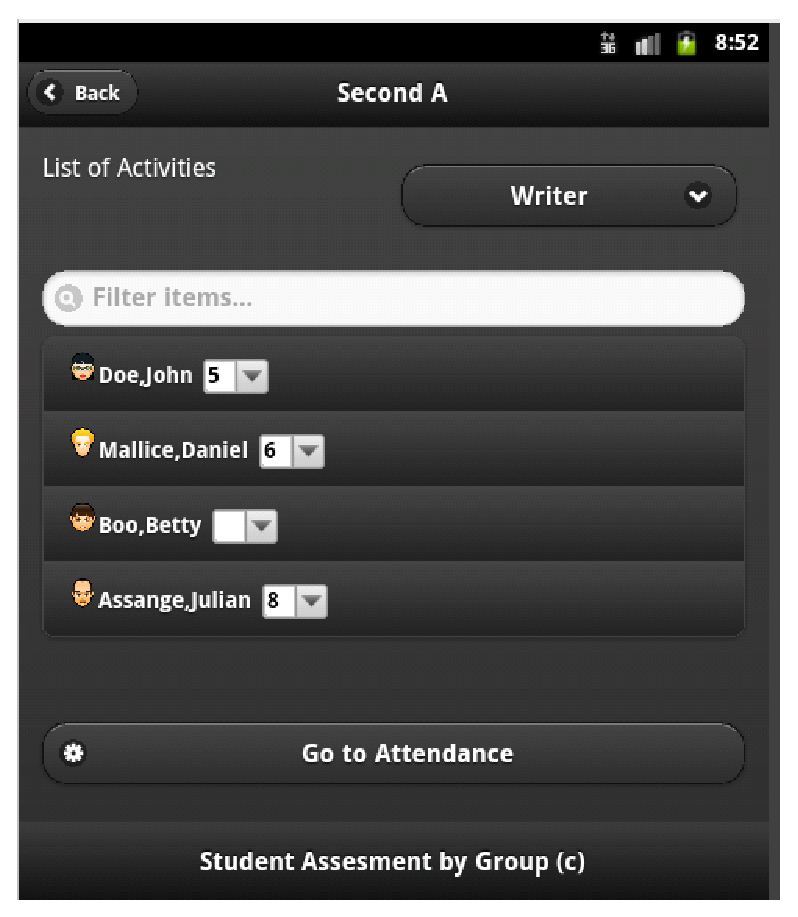
\includegraphics{eduxes_students_assessment01.eps}
        \caption{Assessment}
        \label{fig:EduXesAssessment}
    \end{center}
\end{figure}



\begin{figure}
    \begin{center}
        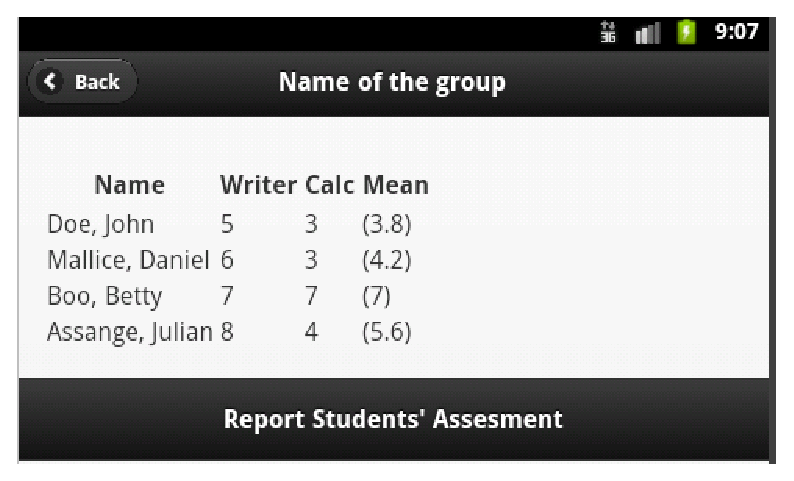
\includegraphics{eduxes_assessment1.eps}
        \caption{ Assessment Report}
        \label{fig:EduXesAssessmentReport}
    \end{center}
\end{figure}


%  i) Timetable for actual date: list of groups for selected day.

%  j) Add attendance, misbehaviour for each student. Student attendance, misbehaviour, punctuality are set here.
% Tasks to be done
%  k) Add error handling. Error handling is managed throw dbErrorFunc.
%  l) Retrieve and insert data from and to database. 
%  m) List of attendance, misbehaviour incidents. A list of attendance will be carried on, reusing Siestta interfaces.
%  n) Add activities grades for each student. 
%  o) List students marks and final mark. On a window, group, student name and surname will be shown, and a table with his/her marks.
%  p) Activities management window. Add, remove and update activities. It includes name of activity and percent weight.
%  q) Management of student notes. Student's notes could be included as an option.
%  r) List of student notes. In a table-like window, notes will be displayed.
% ).
% Make a group management window.
%  h) Students: These pages are not active.
% Make list of students window.
% Students management window (insert-update-delete students)
%  i) Timetable for actual date: list of groups for selected day.
% Below queryScheduleSuccess() and querySchedulePerDayDB() functions are written, these functions fills daily_schedule page as shown in Illustration 6: Application Skeleton.
% 

% 
%  j) Add attendance, misbehaviour for each student. Student attendance, misbehaviour, punctuality are set here.
% Tasks to be done
%  k) Add error handling. Error handling is managed throw dbErrorFunc.
%  l) Retrieve and insert data from and to database. 
%  m) List of attendance, misbehaviour incidents. A list of attendance will be carried on, reusing Siestta interfaces.
%  n) Add activities grades for each student. 
%  o) List students marks and final mark. On a window, group, student name and surname will be shown, and a table with his/her marks.
%  p) Activities management window. Add, remove and update activities. It includes name of activity and percent weight.
%  q) Management of student notes. Student's notes could be included as an option.
%  r) List of student notes. In a table-like window, notes will be displayed
% 
% 
% 
% 


%%%%%%%%%%%%%%%%%%%%%%%%%%%%%%%%%%%%%%%
%% sqlt-diagram -d MySQL  --color  -t "EduXes Database" -o data_base.png  DATABASE.sql
%%

\newpage
\section{Database \label{DataBase}}
Next figure \ref{fig:Database} is a graphical representation of EduXes database \ref{DatabaseSchema} obtained using \textit{sqlfairy} program \cite{SQLFairy}.
\begin{figure}
    \begin{center}
        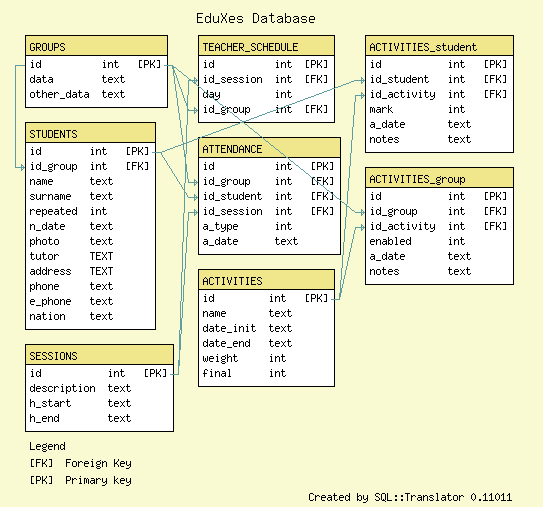
\includegraphics[width=\textwidth]{data_base.png}
        \caption{Database}
        \label{fig:Database}
    \end{center}
\end{figure}

\begin{bclogo}[couleur=green!30,arrondi=0.1, logo=\bcpanchant,  ombre=true ] 
{EduXes Database structure \label{DatabaseSchema}}   
\begin{verbatim}
-- Groups
CREATE TABLE IF NOT EXISTS GROUPS (id  integer primary key ,
    data text , other_data text);
--- Students
CREATE TABLE IF NOT EXISTS STUDENTS (
      id integer primary key, id_group integer not null,
       name text, surname text,
      repeated integer, n_date text , photo text,
      tutor TEXT, address TEXT, phone text, e_phone text,
       nation text,
      FOREIGN KEY(id_group) REFERENCES GROUPS(id));
-- Sessions ( franja horaria)
CREATE TABLE IF NOT EXISTS SESSIONS (id  integer primary key,
        description text, h_start text, h_end text);
-- Teacher's schedule
CREATE TABLE IF NOT EXISTS TEACHER_SCHEDULE (id  integer primary key,
      id_session integer, day integer, id_group integer,
      FOREIGN KEY(id_group) REFERENCES GROUPS(id),
      FOREIGN KEY(id_session) REFERENCES SESSIONS(id));
-- Students Attendance
CREATE TABLE IF NOT EXISTS ATTENDANCE (id integer primary key ,
      id_group integer, id_student integer, id_session integer,
      a_type integer, a_date text,
      FOREIGN KEY (id_student) REFERENCES STUDENTS (id),
      FOREIGN KEY (id_group) REFERENCES GROUPS(id),
      FOREIGN KEY (id_session) REFERENCES SESSIONS(id) );
-- Activities
CREATE TABLE IF NOT EXISTS ACTIVITIES
    (id integer primary key, name text, date_init text, 
    date_end text, weight integer, final integer );
CREATE TABLE IF NOT EXISTS activities_student
    (id integer primary key ,  id_student integer,
     id_activity integer,
    mark integer, a_date text, notes text,
    FOREIGN KEY (id_student) REFERENCES students (id),
    FOREIGN KEY (id_activity) REFERENCES activities(id) );
CREATE TABLE IF NOT EXISTS activities_group
    (id integer primary key ,  id_group integer,
     id_activity integer,
    enabled integer, a_date text, notes text,
    FOREIGN KEY (id_group) REFERENCES groups (id),
    FOREIGN KEY (id_activity) REFERENCES activities(id) );
\end{verbatim}
\end{bclogo}
